\chapter{Datensatz}

Wie bereits in Chapter \ref{einleitung} erwähnt, wird der InterHand2.6M Datensatz \cite{InterHand} genutzt.
Dabei handelt es sich um Bilder von Händen, die zeitgleich von 6 verschieden Kameras aus unterschiedlichen Perspektiven aufgenommen wurden. \\
\begin{figure}[!htb]
    \centering
    \fbox{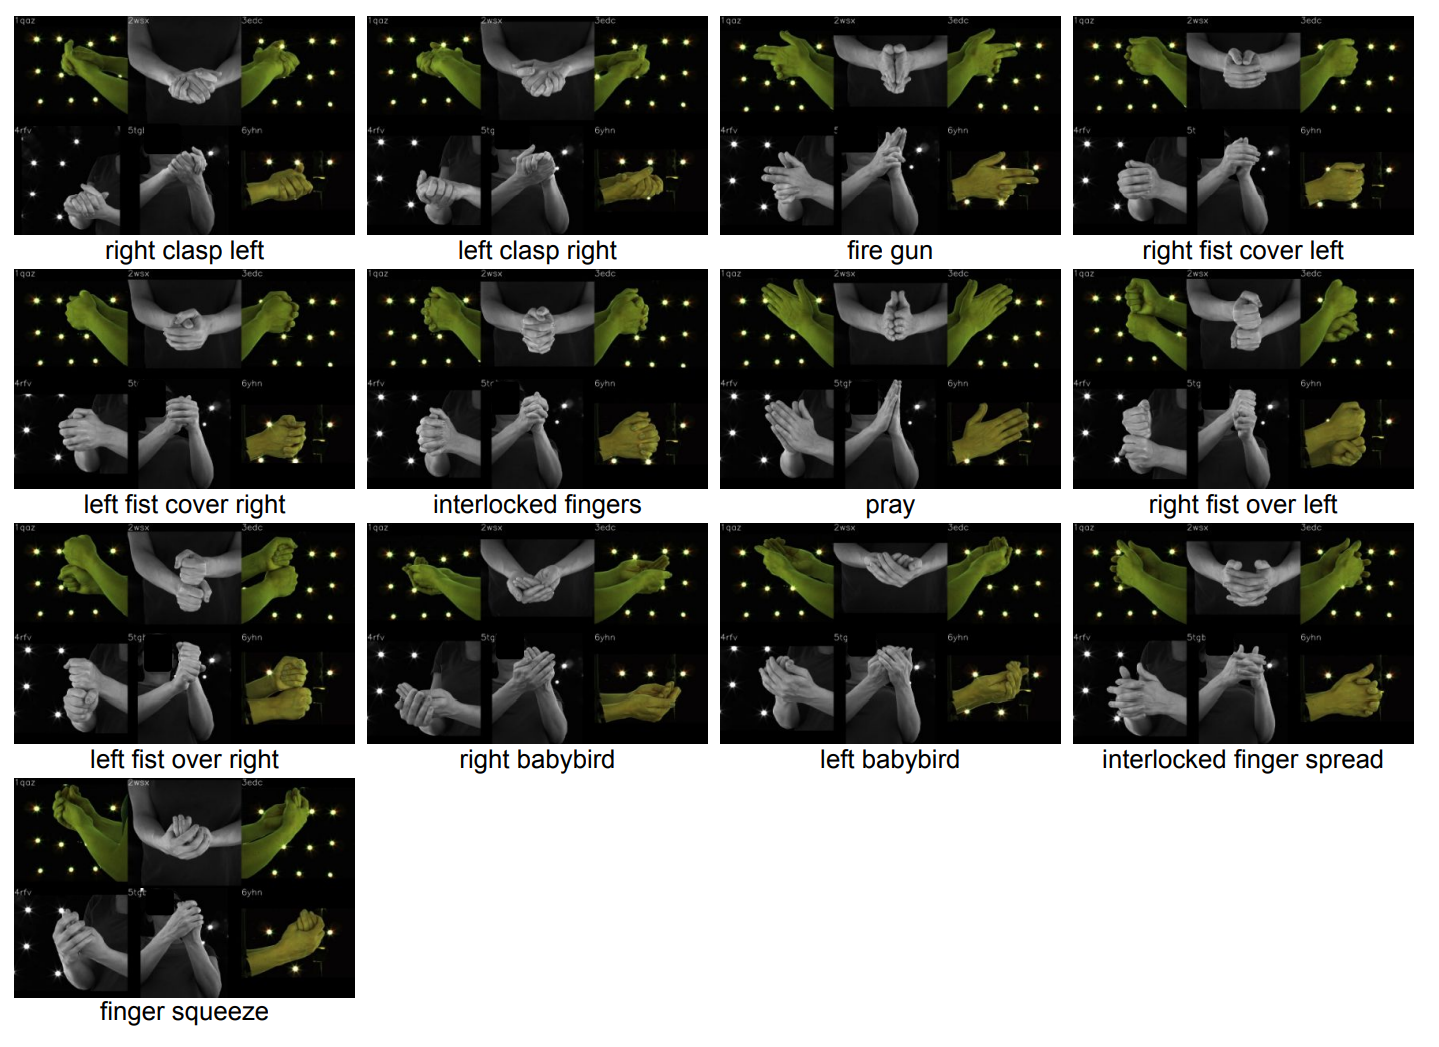
\includegraphics[width=15.5cm]{abbildungen/interhand26.PNG}}
    \caption{Beispiele InterHand2.6M Bilder\cite{InterHand}}
    \label{fig:interhand}
\end{figure} 

Hierbei kann es sich um eine rechte, eine linke oder aber auch um ein paar interagierender Hände handeln.
Abbildung \ref{fig:interhand} zeigt einige Posen von interagierenden Händen aus den 6 verschiedenen Blickwinkeln.
Um als interagierend gelabelt zu werden, müssen lediglich 2 Hände auf dem Bild sein, egal ob diese sich berühren oder nicht. 
Eine mögliche Erklärung dafür ist, dass je nach Blickwinkel die Hände auf dem Bild überlappt dargestellt sind, es jedoch zu aufwändig ist, jeden Blickwinkel manuell zu prüfen. 
Der ganze Prozess wird dadurch also vereinfacht. \newline
Der Datensatz wurde als Video aufgenommen und in einzelne Bilder zerlegt.
Für das Projekt wurde die 5fps (1 Sekunde Video wird zu 5 Bildern umgewandelt) Variante ausgewählt.
Diese enthält nur 1/6 der Bilder der 30fps Variante, jedoch sind es immer noch 2,6 Millionen Bilder, die sich mehr unterscheiden als die der 30fps Variante. \newline
Von den knapp 2,6 Millionen Bildern wurden  650.000 von Menschen annotiert, wohingegen der Rest durch Maschinen errechnet wurde (z.B. durch die unterschiedlichen Kamerablickwinkel). 
Der Fokus der menschlichen Annotierung lag dabei auf den interagierenden Händen, vermutlich da die Komplexität (durch z.B. Überlappung) höher ist.
Von den 1,4 Millionen Bildern einzelner Hände wurden ca. 170.000 Bilder menschlich annotiert ($\sim$ 12\%), wohingegen von den 1,2 Millionen interagierenden Händen ca. 475.000 menschlichen Ursprungs ($\sim$ 40\%) sind. 
Erwähnenswert ist auch, dass bei den interagierenden Händen, welche von Maschinen annotiert wurde, ist teilweise nur eine Hand gelabelt.
Die Keypoints der zweiten Hand sind außerhalb des Bildes. \\
Eine Aufteilung in Train (1.360.000 Bilder, $\sim$52\%), Val (380.000 Bilder, $\sim$15\%) und Test (850.000 Bilder, $\sim$33\%) liegt bereits vor und wird auch im weiteren Verlauf so genutzt.
